\documentclass{article}
\usepackage{style}
\usepackage{MyNotations}
\begin{document}

\newpage 
\section{Kinematics of Burgers vector conservation}
\subsection{Dislocation transport equation}

\begin{figure}[H]
    \centering
    \begin{subfigure}{.45\textwidth}
      \centering
      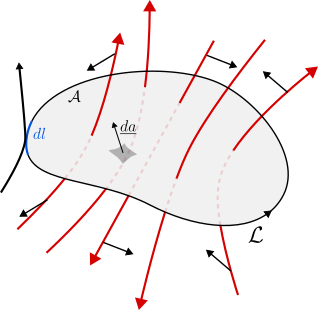
\includegraphics[width=0.65\textwidth]{imgs/fdm/flux.png}
      \caption{A bundle of dislocation lines threading through a patch $\mathcal{A}$, delimited by a closed curve $\mathcal{L}$.}
      \label{fig:flux}
    \end{subfigure}%
    \hspace*{1cm}
    \begin{subfigure}{.45\textwidth}
      \centering
      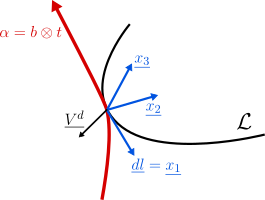
\includegraphics[width=0.75\textwidth]{imgs/fdm/localfram.png}
      \caption{A local frame analysis of a dislocation line  crossing the boundary $\mathcal{L}$ with velocity $\vecc V^d$.}
    \label{fig:localframe}

    \end{subfigure}
    \caption{Illustration of Burgers vector transport through a patch $\mathcal{A}$}
    \end{figure}
The idea behind Burgers vector conservation, in the case of moving dislocations is to introduce a balance law of the type:
\begin{center}
    \emph{Rate of change = what comes in - what comes out}
\end{center}
For that, we consider an area patch $\mathcal{A}$, delimited by a closed curve $\mathcal{L}$. The Burgers vector content can be thought of as bundle of lines each carrying a given Burgers vector $\vecc{b}$ entering or exiting the surface $\mathcal{A}$, see \cref{fig:flux}. As dislocations move with a velocity field $\vecc{v^d}$, the rate of change of the Burgers vector content is given as follows:
\begin{equation}
    \frac{\partial}{\partial t}\left[ \int_{\mathcal{A}(t)} \Tens{\alpha}\,\vecc{n}\: da \right]
\end{equation}
Note that the integration is performed over an evolving area $\mathcal{A}(t)$ (so it its boundary $\mathcal{L}(t)$).\\
The main conceptual idea is that since the Burgers vector is constant along each individual dislocation line, how dislocation lines evolve within the patch does not matter and does not affect the rate of the change of dislocations content. What really contributes is the Burgers information crossing the contour $\mathcal{L}(t)$, i.e leaving or entering the patch $\mathcal{A}(t)$. For that we have to integrate, along the closed curve, elementary contributions on each infinitesimal element $\vecc{dl}$. This contribution should extract only the Burgers vector content that crossed the element and left/entered the area. If we denote by $f$ the flux of Burgers vector crossing an element $\vecc{dl}$ along $\mathcal{L}$, then the conservation law of Burgers content becomes:
\begin{equation}\label{eq:balance0}
    \frac{\partial}{\partial t}\left[ \int_{\mathcal{A}(t)} \Tens{\alpha}\,\vecc{da} \right] = \oint_{\mathcal{L}(t)} f\, \vecc{dl}
\end{equation}
At this step, Burgers vector flux $f$ can be either a scalar or a second order tensor so that the R.H.S of the previous equation yields a vector to be integrated over the closed curve.\\

A local analysis in a simple case of this statement comes as following:\\
Consider an infinitesimal curve element $\vecc{dl}$, crossed by a dislocation line with tangent vector $\vecc{t}$ and carrying a Burgers vector $\vecc{b}$, see \cref{fig:localframe} . The dislocation line moves with a velocity $\vecc{v^d}$ with respect to the material. Clearly, if $\vecc{v^d}$ is parallel to $\vecc{t}$, no flux is generated, because $\vecc{b}$ is constant along the dislocation line and the line doesn't end within the body. Also, obviously if $\vecc{v^d}$ is parallel $\vecc{dl}$, no flux is generated, because nothing leaves the patch $\mathcal{A}$.\\

$\bm{\Rightarrow}$ This means that Brugers flux is generated iff $\vecc{v^d}$ is perpendicular to both $\vecc{t}$ and $\vecc{dl}$. Or in other words, only perpendicular components of $\vecc{v^d}$ to both vectors generate some Burgers flux.\\

Mathematically, this is performed using mixed product $\vecc{v^d}\cdot (\vecc{t} \times \vecc{dl}) $, which projects the velocity $\vecc{v^d}$ on the normal vector $\vecc{t} \times \vecc{dl}$. To exhibit $\vecc{dl}$, we use the circular shift of triple product:
\begin{equation}
\vecc{v^d}\cdot (\vecc{t} \times \vecc{dl}) =  (\vecc{v^d}\times \vecc{t})\cdot \vecc{d_l} = -( \vecc{t} \times \vecc{v^d})\cdot \vecc{d_l}
\end{equation}
This motivates the tensorial form of the previous statement in order to incorporate all possible directions crossing $\vecc{dl}$. We define the dislocation density flux tensor as :
\begin{equation}
    \Tens{f} = - \Tens{\alpha} \times \vecc{v^d}
\end{equation}
Let's stop for a moment to understand the cross product between a second order tensor and vector field. In fact, the quantity $\Tens{\alpha} \times \vecc{v^d}$ is a new second order tensor whose lines are vectors given by the cross product of each line of the $\Tens{\alpha}$ in it matrix form with the vector field $\vecc{v^d}$. This is best seen in indicial notation:
\begin{equation}
    \Tens{\alpha} \times \vecc{v^d} = \underbrace{\Levi{jkl} \alpha_{ik} v^d_{l} }_{(\vecc{[\alpha]^i} \times \vecc{v^d})\cdot \unitvec{i}}\unitvec{i} \otimes \unitvec{j}
\end{equation}
Where, $[\alpha]^i$ is meant to represent line $i$ in matrix' representation of $\Tens{\alpha}$. Intuitively, a line $i$ in  represents, crudely, all components of tangent vectors whose corresponding burgers vector is along $\unitvec{i}$. In this optic, the Burgers flux density $f$ previously introduced will have a tensorial nature :
\begin{equation}
    \Tens{f}= -\Tens{\alpha} \times \vecc{v^d}
\end{equation}
So that the RHS of \cref{eq:balance0}, will act as mixed product for all directions: each line of $\Tens{\alpha}$ is crossed with $\vecc{v^d}$ and then dotted with $\vec{dl}$ to extract normal components along each directions (these are the only contributions to any change in Burgers vector content). We write as \parencite{acharyaMicrocanonicalEntropy2011} (Appendix B):
\begin{equation}
    \frac{\partial}{\partial t}\left[ \int_{\mathcal{A}(t)} \Tens{\alpha}\,\vecc{da} \right] = - \oint_{\mathcal{L}(t)} \Tens{\alpha}\times \vecc{v^d} \:\vecc{dl}
\end{equation}
This derivation was influenced the discussion \parencite{fressengeasMechanicsdislocation2017}.
A different construction is suggested by \parencite{muraContinuousdistribution1963}, by \parencite{foxContinuumTheory1966} and by \parencite{kosevichDYNAMICALTHEORY}. We focus on the later in the following section.
\subsection{Kosevich's construction}
In his work \parencite{kosevichDYNAMICALTHEORY}, \emph{Kosevich} argues that in the case of moving dislocations, the spatial gradient of the material velocity field $\partial v_k/ \partial x_i$  and time derivative of the elastic distortion $\partial w_{ik} / \partial t$ are not equal ( with $u_{ik} = \partial u_k / \partial x_i$). They are equal in the absence of dislocations. So in general, when dislocation are involved, we have:
\begin{equation}
    \frac{\partial v_k}{\partial x_i} \neq \frac{\partial u_{ik}}{\partial t}
\end{equation}
It is important to note here the similarity with the phase field crystal, if the same scalar field is used to describe mass
He introduces a tensor field $j_{ik}$ to balance these two quantities. He calls $j_{ik}$ the dislocation flux density and He writes:
\begin{equation}\label{eq:Kosevichconsflux}
   \frac{\partial u_{ik}}{\partial t} = \frac{\partial v_k}{\partial x_i}  - j_{ik}
\end{equation}
For compatibility reasons, he states that:
\begin{equation}
\partial_t \Tens{\alpha}+ \Trot{\Tens{j}} =0
\end{equation}
He also shows that, at least, locally, a flux of Burgers vector is generated iff the velocity is perpendicular to both tangent to a curve and to the dislocation line:
\begin{equation}
    j_{ik} = N \mathcal{E}_{ilm}t_lb_kV_m \quad \sim \Tens{\alpha} \times \vecc{v^d}
\end{equation}
In addition, in his work, states that the total geometric distortion $U_{ik}$ (and not the elastic distortion) is actually equal to the gradient of the velocity field .
\begin{equation*}
     \frac{\partial v_k}{\partial x_i} = \frac{\partial U_{ik}}{\partial t}
\end{equation*}
Replacing $\partial v_k/\partial x_i$ by \ref{eq:Kosevichconsflux}, we write that:
\begin{equation}
    \frac{\partial v_k}{\partial x_i} = \frac{\partial }{\partial t} \left(U_{ik}-u_{ik}\right) = \partial_t u^{pl}_{ik} \quad \text{with } \quad u^{pl} \equiv U-u
\end{equation}
Which means that $j_{ik}$ is linked to the rate of plastic distortion in the medium. \\

Acharya in 2011, in annex B, he restates the conservation of Burgers vector in case of a moving dislocation distribution. The localization of the conservation of Burgers vector yields two main results: An evolution law for $\Tens{\alpha}$ and an additive decomposition of $\Tens{L}$ which was only seen in his work in 2015.

\subsection{Evolution law of dislocation density tensor :}
Burgers vector balance law states that :
\begin{equation}\label{eq:balanceBurgINT}
    \frac{\partial}{\partial t}\left[ \int_{\mathcal{A}(t)} \Tens{\alpha}(\vecc{x},t)\,\vecc{da} \right] = - \oint_{\mathcal{L}(t)} \Tens{\alpha}\times \vecc{v^d} \:\vecc{dl}
\end{equation}
Using Stokes-theorem, one can write :
\begin{equation}
    \frac{\partial}{\partial t}\left[ \int_{\mathcal{A}(t)} \Tens{\alpha}(\vecc{x},t)\,\vecc{da} \right] = - \int_{\mathcal{A}(t)} \Trot{\Tens{\alpha}\times \vecc{v^d}} \:\vecc{da}
\end{equation}
\subsubsection{Small deformations :}
In the case of small deformations, one can assume that approximately $\mathcal{A}(t)\approx \mathcal{A}_0$ is invariant. The time derivative goes inside the integral and we get by localization theorem:
\begin{equation}
    \dot{\Tens{\alpha}} = - \Trot{\Tens{\alpha}\times \vecc{v^d}}
\end{equation}
Which yields the evolution law of the dislocation density $\Tens{\alpha}(\vecc{X},t)$.
 \subsubsection{Finite deformations :}
In the case of Finite deformations, the time derivative cannot be inverted with the integration operation since the domain is time variant.
The remedy to this, is to pull-back everything to the initial (as-received) configuration using Nanson formula: $\vecc{da}= J\Tens{F}^{-t}\vecc{dA}$ and the tranformation mapping $\varphi(\vecc X,t)$
\begin{equation*}
  \frac{\partial}{\partial t}\left[ \int_{\mathcal{A}_0} J\Tens{\alpha}(\varphi\left(\vecc{X},t\right),t)\Tens{F}^{-t}\,\vecc{dA} \right] = - \int_{\mathcal{A}_0} J \Trot{\Tens{\alpha}\times \vecc{v^d}}\: \Tens{F}^{-t} \:\vecc{dA}
\end{equation*}
Were, explicitly Highlight the fact that the fields depend on the Lagragian variable $\vecc{X}$.\\
Inverting the integration and time derivation then localizing yields the following result:
\begin{equation*}
    \frac{\partial}{\partial t}\left[J\Tens{\alpha}(\varphi\left(\vecc{X},t\right),t)\Tens{F}^{-t}\right] = - J \, \Trot{\left(\Tens{\alpha}\times \vecc{v^d}\right) }\: \Tens{F}^{-t}
\end{equation*}
The LHS can be expanded : 
\begin{equation}\label{eq:derivationexpansion}
    \frac{\partial}{\partial t}\left[J\Tens{\alpha}(\varphi\left(\vecc{X},t\right),t)\Tens{F}^{-t}\right] = \dot J \Tens{\alpha}\:\Tens{F}^{-t} + J \dot{\Tens{\alpha}}\:\Tens{F}^{-t}  +J \Tens{\alpha}\: \dot{\Tens{F}^{-t}}= - J \, \Trot{\left(\Tens{\alpha}\times \vecc{v^d}\right) }\: \Tens{F}^{-t}
\end{equation}
where $\dot{\Tens{\alpha}}$ is the material derivative.\\
Now, we investigate all time derivatives involved in the previous equation. The first terme involving $\dot J$, can be easily computed using the mass conservation laws: (recall that  $\vecc{x} = \varphi(\vecc X,t)$)
\begin{equation*}
    \text{Lagragian : } \rho_0(\vecc X) = J(\vecc X,t) \rho(\vecc x,t) \qquad \qquad \text{Eulerian : } \dot{\rho} +\rho \,\vdiv \vecc{v}=0
\end{equation*}
Derivating the Lagragian balance law and replacing $\dot \rho$ with its expression from the Eulerian law gives:
\begin{equation}\label{eq:Jdot}
    0=\dot J \rho + J\dot \rho  \quad \Rightarrow \quad \boxed{\dot J = J \vdiv \vecc v = J \Tr{L}}
\end{equation}
For the last term in \ref{eq:derivationexpansion}, one easily obtains (Since transposition is commutative with derivation and inversion):
\begin{equation}\label{eq:F-tdot}
    \Tens{F}\,\Tens{F}^{-1} = \Tens{I}_3 = \quad \Rightarrow \quad \underbrace{\dot{\Tens{F}}\,\Tens{F}^{-1}}_{=\Tens{L}}+ \Tens{F}\,\dot{\Tens{F}^{-1}}=0 \quad \Rightarrow \quad \boxed{\dot{\Tens{F}^{-t}} = - \Tens{L}^{t}\Tens{F}^{-t}}
\end{equation}
With this two elements, we replace \ref{eq:F-tdot} and \ref{eq:Jdot} in \ref{eq:derivationexpansion}. Hence, we find:
\begin{equation}\label{eq:evoluionalpha_material}
\boxed{(\vdiv{\vecc{v}} )\, \Tens{\alpha} + \dot{\Tens{\alpha}}-\Tens{\alpha}\,\Tens{L^{t}} = - \Trot{\Tens{\alpha}\times \vecc{v^d}}}
\end{equation}
Because $J=det \Tens{F} \neq 0$.\\
We expand the material derivative:
\begin{equation}
    \dot{\Tens{\alpha}} = \partial_t \Tens{\alpha} + (\Tgrad{\Tens{\alpha}}) \cdot \vecc{v} 
\end{equation}
The evolution law of the dislocation density tensor becomes:
\begin{equation}\label{eq:evolutionEXPANDED}
    \partial_t \Tens{\alpha} + (\Tgrad{\Tens{\alpha}})\cdot \vecc{v} +(\vdiv{\vecc{v}} )\, \Tens{\alpha} -\Tens{\alpha}\,\Tens{L^{t}} = - \Trot{\Tens{\alpha}\times \vecc{v^d}}
\end{equation}
A simple identity yields :
\begin{equation}
    (\Tgrad{\Tens{\alpha}})\cdot \vecc{v} +(\vdiv{\vecc{v}} )\, \Tens{\alpha} -\Tens{\alpha}\,\Tens{L^{t}} = \Trot{\Tens{\alpha}\times \vecc{v^d}}
\end{equation}
with can be easily proven in indicial notations:
\begin{align*}
    \left[(\Tgrad{\Tens{\alpha}})\cdot \vecc{v} +(\vdiv{\vecc{v}} )\, \Tens{\alpha} -\Tens{\alpha}\,\Tens{L^{t}}\right]_{ij} &= \alpha_{ij,k} v_k+v_{k,k}\alpha_{ij}-\alpha_{ik}v_{j,k}\\
        &= (\alpha_{ij}v_k)_{,k}-(\alpha_{ik}v_j)_{,k} \quad \text{because} \quad \alpha_{ik,k}=0 \quad( \Tdiv\,\Tens{\alpha} = 0)
\end{align*}
We note that, in components form:
\begin{align*}
   \left[ \Trot \Tens{\alpha}\times \vecc{v} \right]_{ij}&= \mathcal{E}_{lkj}(\Tens{\alpha}\times \vecc{v})_{ik,l} \\
    &=\mathcal{E}_{lkj}(\alpha_{in}v_m\mathcal{E}_{nmk})_{,l} \\
        &=\mathcal{E}_{lkj}\mathcal{E}_{nmk}(\alpha_{in}v_m)_{,l}\\
        &=\mathcal{E}_{jlk}\mathcal{E}_{nmk}(\alpha_{in}v_m)_{,l}\\
        &=\left(\kron{j}{n}\kron{l}{m}- \kron{j}{m}\kron{l}{n}\right)(\alpha_{in}v_m)_{,l}\\
        &=\kron{j}{n}\kron{l}{m}(\alpha_{in}v_m)_{,l} -\kron{j}{m}\kron{l}{n}(\alpha_{in}v_m)_{,l}\\
        &= (\alpha_{ij}v_m)_{,m}-(\alpha_{il}v_j)_{,l}
\end{align*}
This proves THE IDENDITY :
\begin{equation}\label{eq:identityCurl}
    (\Tgrad{\Tens{\alpha}})\cdot \vecc{v} +(\vdiv{\vecc{v}} )\, \Tens{\alpha} -\Tens{\alpha}\,\Tens{L^{t}} = \Trot \Tens{\alpha}\times \vecc{v}
\end{equation}
Replacing \ref{eq:identityCurl} in \ref{eq:evolutionEXPANDED}, yields:
\begin{equation}\label{eq:Evolutionalpha_Eulerian}
    \boxed{\partial_t \Tens{\alpha} + \Trot (\Tens{\alpha}\times (\vecc{v^d}+ \vecc{v})) =0}
\end{equation}
\subsubsection{Additive decomposition of velocity gradient tensor:}
Another way to localize the Brugers vector balance law, would be to forumlate it in terms of the inverse elastic distortion $\Tens{W}$. We recall that the dislocation density tensor $\Tens{\alpha}$ is defined as:
\begin{equation*}
    \Tens{\alpha} = - \Trot \Tens{W}
\end{equation*}
Replacin in Brugers vector Conservation Law \ref{eq:balanceBurgINT}, one finds :
\begin{equation*}
    \frac{\partial}{\partial t}\left[ \int_{\mathcal{A}(t)} \Trot \Tens{W}\,\vecc{da} \right] =  \oint_{\mathcal{L}(t)} \Tens{\alpha}\times \vecc{v^d} \:\vecc{dl} \quad \xRightarrow[\text{Theorem}]{\text{Stokes}} \quad     \frac{\partial}{\partial t}\left[ \int_{\mathcal{L}(t)} \Tens{W}\,\vecc{dl} \right] =  \oint_{\mathcal{L}(t)} \Tens{\alpha}\times \vecc{v^d} \:\vecc{dl}
\end{equation*}
One can can be tempted to pull back to the initial configuration, as previously done, but $\dot{\Tens{W}}$ is ill defined on the initial configuration. As a remedy to this issue, Acharya 2004, suggests to fix an instant in time, say $t$, in which we wich to evalulat the quantities. Starting from time $t$, the motion is now parametrized by a new variable $\tau \in [ t ,+ \infty [ $. We denote by $\Tens{F_\tau}$, the deformation gradient associated with the motion from $t$ to $t + \tau$. \\
We evaluate the previous equation at time $\tau$, and we explicitly write a $\tau$ subsccript to indicate the time.
\begin{equation}
    \frac{\partial}{\partial t}\left[ \int_{\mathcal{L}(\tau)} \Tens{W}\,\vecc{dl_{\tau}} \right] =  \oint_{\mathcal{L}(\tau)} \Tens{\alpha}\times \vecc{v^d} \:\vecc{dl_{\tau}}
\end{equation}
This can now be pulled back, to the configuration at time $\tau$, using $\Tens{F_\tau}$: (As if, in the new parametrization, time $t$ is the initial configuration).
\begin{equation}
    \frac{\partial}{\partial t}\left[ \int_{\mathcal{L}(t)} \Tens{W}\,\Tens{F_\tau}\, \vecc{dL_{t}} \right] =  \oint_{\mathcal{L}(t)} \Tens{\alpha}\times \vecc{v^d} \:\Tens{F_\tau}\, \vecc{dL_{t}} \quad \Rightarrow \quad \int_{\mathcal{L}(t)} \dot{\overline{\Tens{W}\,\Tens{F_\tau}}}\, \vecc{dL_{t}}  =  \oint_{\mathcal{L}(t)} \Tens{\alpha}\times \vecc{v^d} \:\Tens{F_\tau}\, \vecc{dl_{t}}
\end{equation}
Since localization theorem doesn't hold along arbitrary curves, we use Stokes theorem to switch into surface integration:
\begin{equation}
    \int_{\mathcal{A}(t)} \Trot \! \left( \dot{\overline{\Tens{W}\,\Tens{F_\tau}}} - \Tens{\alpha}\times \vecc{v^d} \Tens{F_\tau}\right) \vecc{da_t}=0
\end{equation}
Using the localization theorem, and ignorning any additive gradient of some vector field ($\Trot \nabla \vecc{f} = 0 \: \forall \vecc{f}$), one writes :
\begin{equation}
    \dot{\overline{\Tens{W}\,\Tens{F_\tau}}} = \Tens{\alpha}\times \vecc{v^d} \Tens{F_\tau}
\end{equation}
Ignorning the additional $\nabla \vecc f$, is justified by the fact thet localization is a microscopic statement and at a microscopic level, plastic deformation can only occur due to dislocation motion: the term $\Tens{\alpha}\times \vecc{v^d}$ is responsible for that. Arranging the terms gives : ($\dot{(\:)}$ is the material derivative)
\begin{equation}
    \dot{\Tens{W}}\Tens{F_\tau} + \Tens{W} \Tens{L_{\tau}}  \Tens{F_\tau} =(\Tens{\alpha}\times \vecc{v^d} ) \Tens{F_\tau}
\end{equation}
Evaluating at $\tau=0$ yields the desired result: $(\Tens{F_\tau}=\Tens 1)$
\begin{equation}\label{eq:EvolutionW}
    \boxed{\dot{\Tens{W}} + \Tens{W} \Tens{L}  =\Tens{\alpha}\times \vecc{v^d}  }
\end{equation}
This statement, it appears to me in spirit, as a large deformation generlization of Kosevich's observation that time derivative of elastic distortion and the spatial gradient of the velocity field do not balance with each other when dislocation are moving.\\
In his work, Acharya 2015, shows an intersting result by an easy algebraic manupulation of \ref{eq:EvolutionW}. In fact, $\Tens{W}  = \Tens{F_e}^{-1}$, and we can isolate $\Tens L$ from the previous equation:
\begin{equation}
    \Tens{L}=- \Tens{F_e} \dot{\Tens{F_e}^{-1}} + (\Tens{F_e}\Tens{\alpha})\times \vecc{v^d}
\end{equation}
But, as seen previously
\begin{equation}
    \Tens{F_e}\,\Tens{F_e}^{-1} = \Tens{I}_3 = \quad \Rightarrow \quad \dot{\Tens{F_e}}\,\Tens{F_e}^{-1}+ \Tens{F_e}\,\dot{\Tens{F_e}^{-1}}=0 \quad \Rightarrow \quad \dot{\Tens{F_e}}\,\Tens{F_e}^{-1}=- \Tens{F_e}\,\dot{\Tens{F_e}^{-1}}
\end{equation}
Finally,
\begin{equation}
    \boxed{
        \Tens{L}=\underbrace{\dot{\Tens{F_e}}\,\Tens{F_e}^{-1}}_{\Tens{L_e}} + \underbrace{(\Tens{F_e}\Tens{\alpha})\times \vecc{v^d}}_{\Tens{L_p}}
    }
\end{equation}
This may be interpreted as a fundamental additive decomposition of
the velocity gradient into elastic part $\Tens{L_e}$ and plastic part $\Tens{L_p}$.
The latter is defined by the rate of deformation produced by the flow of dislo-
cation lines in the current configuration, without any reference to the notion of
a pre-assigned reference configuration or a total plastic deformation from it. We bypassed any need of multiplicative decomposition of the gradient of deformation.
\section{Constitutive analysis}
Following Colleman-Noll procedure XXX
\subsection{Mass balance}
\subsection{Momentum balance}
\subsection{Energy Balance}
\subsection{Entropy imbalance}
Starting from the $2^{nd}$ principle of thermodynamics, the entropy density $\eta$ must satisfy :
\begin{equation}
    \frac{d}{dt} \left[\int_\Omega \rho \eta \, dv \right] \geq 0
\end{equation}
Using Legendre transformation we introduce Helmholtz free energy density $\psi:=\varepsilon - \eta \theta$. In an isothermal case, the previous inequality is simply equivalent to:
\begin{equation}
    \mathcal{D} = \int_\Omega \rho \dot \varepsilon \, dv - \int_\Omega \dot \psi \, dv \geq 0
\end{equation}
Were $\mathcal{D}$ is the dissipation. Using energy balance, we have $\rho \dot \varepsilon = \Tens \sigma : \Tens L$. So that, the dissipation becomes:
\begin{equation}
    \mathcal{D} = \int_\Omega \Tens \sigma : \Tens L \, dv - \int_\Omega \dot \psi \, dv  \geq 0
\end{equation}
We suppose, in the most general case, that the free energy density $\psi$ is a function of elastic distortion $\Tens W$ and the dislocation density $\alpha$:
\begin{equation}
    \psi := \psi(\Tens W, \Tens \alpha) \quad \Rightarrow \quad \dot \psi = \frac{\partial \psi}{\partial \Tens W} : \dot{\Tens W} + \frac{\partial \psi}{\partial \Tens \alpha} : \dot{\Tens \alpha}
\end{equation}
Using the evolution laws \ref{eq:evoluionalpha_material} and \ref{eq:EvolutionW}, we get :
\begin{equation}
    \dot \psi = \frac{\partial \psi}{\partial \Tens W} : \left( - \Tens{W} \Tens{L}  +\Tens{\alpha}\times \vecc{v^d}\right) + \frac{\partial \psi}{\partial \Tens \alpha}:\left[ -(\Tr{\Tens{L}} )\, \Tens{\alpha} + +\Tens{\alpha}\,\Tens{L^{t}} - \Trot{\Tens{\alpha}\times \vecc{v^d}} \right]
\end{equation}
Let's now manipulate each term to show conjugate variables. We note that:
\begin{equation}
    \frac{\partial \psi}{\partial \Tens W}: \Tens W \Tens L = \Tens{W}^t\, \frac{\partial \psi}{\partial \Tens W}: \Tens L \quad \text{and} \quad     \frac{\partial \psi}{\partial \Tens \alpha}: \Tens \alpha \Tens L^t = \Tens{\alpha}^t \, \frac{\partial \psi}{\partial \Tens \alpha}: \Tens L^t =  \left(\frac{\partial \psi}{\partial \Tens \alpha}\right)^t \, \Tens{\alpha}: \Tens L 
\end{equation}
And that:
\begin{equation}
    \frac{\partial \psi}{\partial \Tens W}: (\Tens{\alpha}\times \vecc{v^d}) = \partial_{\Tens W} \psi_{ij}\mathcal{E}_{jkl}\alpha_{ik}v^d_l =\partial_{\Tens W} \psi_{ij} \alpha_{ik}\mathcal{E}_{jkl}v^d_l  = \left[ \left(\frac{\partial \psi}{\partial \Tens W}\right)^t \Tens \alpha : \Levi{} \right]\cdot \vecc{v^d}
\end{equation} 
In addition to :
\begin{equation}
    \frac{\partial \psi}{\partial \Tens \alpha} : (\Tr{\Tens{L}}) \Tens \alpha =  (\Tr{\Tens{L}}) \left(\frac{\partial \psi}{\partial \Tens \alpha} :  \Tens \alpha \right) = (\Tens 1 : \Tens{L}) \left(\frac{\partial \psi}{\partial \Tens \alpha} :  \Tens \alpha \right)= \left[\left(\frac{\partial \psi}{\partial \Tens \alpha} :  \Tens \alpha \right) \Tens 1 \right]: \Tens{L} 
\end{equation}
Replacing in the definition of $\mathcal{D}$, we get:
\begin{align*}
    \mathcal{D}&= \bigintss_\Omega \left[\Tens\sigma +\rho \Tens{W}^t\, \frac{\partial \psi}{\partial \Tens W}- \rho \left(\frac{\partial \psi}{\partial \Tens \alpha}\right)^t \, \Tens{\alpha} - \rho \left(\frac{\partial \psi}{\partial \Tens \alpha} :  \Tens \alpha \right) \Tens 1  \right]:\Tens L \, dv - \bigintss_\Omega \left[ \rho \left(\frac{\partial \psi}{\partial \Tens W}\right)^t \Tens \alpha : \Levi{} \right]\cdot \vecc{v^d} \, dv\\
    &+ \bigintss_\Omega \frac{\partial \psi}{\partial \Tens \alpha}:\Trot{\Tens{\alpha}\times \vecc{v^d}}  \, dv
\end{align*}
The last term is also re-arranged using the following tensor identity:
\begin{equation}
    \int_\Omega \Tens A: \Trot \Tens B = \int_\Omega \Trot \Tens{A}:\Tens B \, dv - \int_{\partial \Omega} \Tens A : (\Tens B \times \vecc{n} ) \, da
\end{equation}
So, 
\begin{align*}
    \int_\Omega \rho \frac{\partial \psi}{\partial \Tens \alpha}: \Trot{\Tens{\alpha}\times \vecc{v^d}} &= \int_\Omega \Trot\left( \rho \frac{\partial \psi}{\partial \Tens \alpha} \right):\Tens{\alpha}\times \vecc{v^d} \, dv - \int_{\partial \Omega} \rho \frac{\partial \psi}{\partial \Tens \alpha} : \left[(\Tens{\alpha}\times \vecc{v^d}) \times \vecc{n} \right] \, da \\
    &\int_\Omega \left[ \left(\Trot\left( \rho \frac{\partial \psi}{\partial \Tens \alpha} \right) \right)^t\Tens{\alpha}: \Levi{}\right]\cdot \vecc{v^d}  \, dv - \int_{\partial \Omega} \rho \frac{\partial \psi}{\partial \Tens \alpha} : \left[(\Tens{\alpha}\times \vecc{v^d}) \times \vecc{n} \right] \, da
\end{align*}
Finally, we assemble everything :
\small{
\begin{align*}
    \mathcal{D}&= \bigintsss_\Omega \left[\Tens\sigma +\rho \Tens{W}^t\, \frac{\partial \psi}{\partial \Tens W}- \rho \left(\frac{\partial \psi}{\partial \Tens \alpha}\right)^t \, \Tens{\alpha} - \rho \left(\frac{\partial \psi}{\partial \Tens \alpha} :  \Tens \alpha \right) \Tens 1  \right]:\Tens L \, dv - \bigintsss_\Omega \underbrace{\left\lbrace \left[  \rho \left(\frac{\partial \psi}{\partial \Tens W}\right)  - \Trot \left( \rho \frac{\partial \psi}{\partial \Tens \alpha} \right) \right]^t\Tens{\alpha} : \Levi{} \right\rbrace}_{\text{Driving force $f^d$}}\cdot \vecc{v^d} \, dv\\
    &- \bigintsss_{\partial \Omega} \rho \frac{\partial \psi}{\partial \Tens \alpha} : \left[(\Tens{\alpha}\times \vecc{v^d}) \times \vecc{n} \right] \, da \: \geq 0
\end{align*}}
\normalsize
The previous re-arragement exposes the driving force acting on the dislocations (as conjugate to their velocity $\vecc{v^d}$). The driving force $\vecc{f^d}$ is :
\begin{equation}
    \boxed{
    \vecc{f^d} := \left[  \rho \left(\frac{\partial \psi}{\partial \Tens W}\right)  - \Trot \left( \rho \frac{\partial \psi}{\partial \Tens \alpha} \right) \right]^t\Tens{\alpha} : \Levi{}}
\end{equation}
This dissipative inequality give insights as well as constraints on the constitutive prescription of the stress-elastic distortion relationship and on the velocity of dislocations. In the absence of any dislocation, do disspation occurs, and ....
\end{document}